\documentclass{article}
%\textwidth=150mm
\usepackage[left=3cm,right=3cm]{geometry}
\usepackage{amsmath}
\usepackage{hyperref}
\usepackage{graphicx}
\usepackage{listings}
\usepackage[labelfont=bf]{caption}      % bold figure font
\usepackage{todonotes}

\begin{document}
\title{Manual for the exact diagonalization package RLexact \\
Version 4.0}
\author{Kim Lefmann and Sofie Janas, additions by Camilla Buhl Larsen}
\date{\today}
\maketitle
\begin{abstract}
This manual describes the use and function of the program RLexact. The program performs exact diagonalization of quantum spin systems and calculates physical observables. The geometry and interactions in the system to be diagonalized is given through an input file, the contents of which is described closely. The diagonalization can be greatly speeded up by use of the Lanczos algorithm,
which allows diagonalization of $s=1/2$ Heisenberg models containing up to 36 spins (up to 64 spins for high values of the magnetization). 

The extensive appendix in the manual contains information on the program structure, of use for maintenance and further development.
\end{abstract}

\newpage

\tableofcontents

\newpage

\section{Introduction}
This manual is a very brief guide to the function of the software package RLexact and how to use it. 

RLexact \cite{lefmann96} is constructed to perform numerical work within quantum magnetism, in particular for antiferromagnets. It uses the method
of exact diagonalization, either approximative using the Lanzcos algorithm for sparse numerical matrices, or brute force matrix diagonalization. The package calculates numerical observables like energy and magnetization, 
as well as the dynamical neutron scattering structure factor, $S^{\alpha \alpha}({\bf q},\omega)$.

The RLexact package was developed as a side project during the Ph.D.\ studies of Kim Lefmann and Christian Rischel during 1994 and 1995.
It has been used to support a number of neutron scattering studies and has also formed the basis for independent numerical work
related to neutron scattering results. The full publication list of RLexact covers the journal articles \cite{lefmann96,rischel98,lefmann00, lefmann01,juntunen01,ronnow01,ronnow02,zhang02,stone03,fogh15,ring}, as well as the M.Sc.\ theses of Heidi K.\ Nielsen and Karen-Anne Herdal \cite{HKA}, Torsten Tranum-R\o mer \cite{TTR}, Camilla Buhl Larsen \cite{CBL}, Erik Dreier Christensen \cite{EDC} and Sofie Janas \cite{SJ}, as well as the Ph.D.\ thesis work by Astrid Tranum-R\o mer and ongoing Ph.D. thesis work by Sofie Janas.

\subsection{Licence of use}
Use of RLexact as such will only be in form on an agreed collaboration. 
The package is at present {\em neither} open source code, {\em nor} freely available without permission.
The package is likely later to move towards an open source licence after version 4.0.

The code is presently hosted at the DCSC cluster at the University of Copenhagen.

\section{Functions and algorithms} \label{sect:function}
RLexact is most often used for obtaining solutions to problems of $s=1/2$ systems interacting through the Heisenberg Hamiltonian
\begin{equation}
{\cal H} = \sum_{ij} J_{ij} {\bf s}_i \cdot {\bf s}_j . 
\end{equation}
A system of $N$ spins have $(2S+1)^N$ different states - for spins $S=1/2$ this amounts to $2^N$ states.
This is seen easily by using the $s^z$-representation of the spins.
Diagonalization for large values of $N$ quickly becomes a formidable task, as for already $N=20, s=1/2$, we have to 
diagonalize a $10^6 \times 10^6$ Hamiltonian matrix, which when done naively will require tens of Tbytes of memory.

In order to reduce the matrix size and thereby increase the largest possible $N$, a number of tricks are used:
\begin{itemize}
\item To reduce the dimensionality of the matrix, we employ all possible symmetries of the system, including the fact that in
the Heisenberg model the value $S^z = \sum_j s_j^z$ is a good quantum number,
\item We most often use periodic boundary conditions in order to minimize edge effects and to be able to use also translational invariance to create additional symmetries.
\item Since the matrix representation of ${\cal H}$ in the $s^z$-basis contains mostly zeros, we employ the method of sparse matrix diagonalization by means of storing only non-zero matrix elements.
\item We use the approximative Lanzcos algorithm for the diagonalization of the largest systems.
\end{itemize}
The exact information about the interaction between spins and the geometry of the system is given as an input file, described in
section~\ref{sect:input}. We here first describe in more detail the program functionality.

\subsection{The Hamiltonian}
RLexact supports a large variety of different Hamiltonians to diagonalize. 
The generalized RLexact exchange Hamiltonian is written as
\begin{equation}
{\cal H} = \sum_{ij} \left\{ J^z_{ij} s^z_i s^z_j + J^y_{ij} s^y_i s^y_j + J^x_{ij} s^x_i s^x_j \right\} .
\end{equation}
This expression can be transformed into
\begin{equation} \label{eq:H_ex}
{\cal H} = \sum_{ij} \left\{ J^z_{ij} s^z_i s^z_j +  \frac{1}{2} J^{xy}_{ij} \left(  s^+_i s^-_j + s^-_i s^+_j \right)
  +  \frac{1}{2} J^{\rm anis}_{ij} \left(  s^+_i s^+_j + s^-_i s^-_j \right) \right\}
\end{equation}
by using the substitutions $s^\pm = s^x \pm i s^y$, $J^{xy} = (J^x + J^y)/2$, and $J^{\rm anis} = (J^x - J^y)/2$.

A ring exchange term is implemented in RLexact. This term comes from mobile electrons alternating between 4 sites arranged in a square-like geometry. This interaction has the form \cite{ring}.
\begin{equation}
{\cal H}_{\rm ring} = \sum_{ijkl} J_{\rm ring}\left\{ ({\bf s}_i \cdot {\bf s}_j) ({\bf s}_k \cdot {\bf s}_l) +
 ({\bf s}_i \cdot {\bf s}_l) ({\bf s}_k \cdot {\bf s}_j) - ({\bf s}_i \cdot {\bf s}_k) ({\bf s}_j \cdot {\bf s}_l) \right\} ,
\end{equation}
where it is understood that the ring nearest neighbour pairs are $(i,j)$, $(j,k)$, $(k,l)$, and $(l,i)$. 
No 3-spin triangular ring term has been implemented.

In addition, RLexact has dipolar interaction incorporated
\begin{equation}
{\cal H}_{\rm dip} = \sum_{ij} D_{ij} \left\{ {\bf s}_i \cdot {\bf s}_j - 3 ({\bf s}_i \cdot \hat{r}_{ij})({\bf s}_j \cdot \hat{r}_{ij} ) \right\} ,
\end{equation}
where $\hat{r}_{ij}$ is a unit vector in the direction between the two spins and $D_{ij}$ is the dipolar prefactor.
However, the dipole option is presently under repair.

Finally, RLexact includes the Zeeman interaction for fields of arbitrary magnitude and direction
\begin{align}
{\cal H}_{\rm Z}^z = - \sum_j \mathbf{h} \cdot \mathbf{s}_j \\
\end{align}
where in experimental units $|h| = g \mu_{\rm B} B$.\\

All types of interactions can be combined, except that the Zeeman term can be used only for systems where $m$ is not a good quantum number, meaning no m-symmetry.

\subsection{The symmetries}
For reducing the dimensionality of the problem to be solved, we employ a theorem of quantum mechanics. If an operator commute with the Hamiltonian, $[{\cal H}, \hat{A}]$, it is possible to choose eigenstates of the system that are simulteneously eigenstates to ${\cal H}$ and $\hat{A}$, with eigenvalues $E_i$ and $a_i$, respectively. 
If, in turn, it is easy to identify eigenstates to $\hat{A}$, then this can be used to simplify the problem, since matrix elements of ${\cal H}$ between states with different $a$ is automatically zero.

\subsubsection{Translational symmetry}
A much used symmetry for systems with periodic boundary conditions is that of the translational operator, 
in one dimension given by $\hat{T}$. We assume that the Hamiltonian commutes with the translation, $[{\cal H},\hat{T}] = 0$
and that we denote the eigenvalues of $\hat{T}$ by $t$. Pediodic boundary conditions gives that $\hat{T}^N = t^N = 1$, where $N$
the periodicity of the system under translation (in one dimension this becomes the number of spins). The eigenvalues of $\hat{T}$
therefore must fulfill
\begin{equation}
t = \exp (i 2 \pi n/N) = \exp (i 2 \pi k_T) ,
\end{equation}
where $k_T = n_T/N$ and $n_T$ is an integer ranging from $-N/2+1$ to $N/2$ (for even $N$). In RLexact, we represent the eigenvalues
of $\hat{T}$ by the values of $n_T$, and denote them the translational {\em k-values}.\\
Important note: in RLexact the convention is translation cyclically to the left -- it is important to respect this convention for correct cross section calculations.

\subsubsection{Total $S^z$ symmetry}
Another operator used for dimensionality reduction is the total spin value along the $z$-direction:
\begin{equation}
S^z = \sum_j s_j^z ,
\end{equation}
with eigenvalue named $m$. If in (\ref{eq:H_ex}) we have that all $J_{\rm anis} = 0$, then $S^z$ commutes with {\cal H}, 
and $m$ is a good quantum number of the system. Hence, we can separate the diagonalization problem into the subspaces with different $m$-values.\\

$\hat{T}$ obviously commutes with $S^z$, so states can be simultanous eigenvalues of these two operators and ${\cal H}$. For systems in more dimensions it will usually be possible to define translational operators that commute, giving rise to several simultaneous translational q-values. RLexact relies heavily on this fact and allows the user to specify any possible geometric symmetry, relying on the user to ensure that the specified symmetries commute.

\subsubsection{Spin inversion symmetry}
An additional symmetry incorporated into RLexact is the spin inversion symmetry, which simply flips all spins in a given state -- thus, the symmetry is termed the \texttt{spinflip} inside the RLexact code. States in the $m_z=0$ subspace are typically invariant with respect to spin inversion operator, which is defined by the operator $Z$:
\begin{equation}
Z|S_0^z, S_1^z,\dots,S_{N-1}^z\rangle=|-S_0^z, -S_1^z,\dots,-S_{N-1}^z\rangle
\end{equation}
The spin inversion operator has eigenvalues of $\pm 1$. Since it commutes with the $T$ and total $S^z$ operators it can be used to further reduce the dimensionality of the subspace.

\subsection{Representation: Uniques and momentum states}
In RLexact, states are represented by a bit pattern. A long integer is represented by 64 bits, which in turn will mean 64 possible spins.
For example for $N=4$, the bit pattern $| \downarrow \downarrow \uparrow \uparrow \rangle$ is represented by the binary number 0011, or the number 3. The rightmost bit is always indexed 0, and the leftmost bit is indexed $N-1$.\\

Consider now that the $N=4$ system is organized as a linear chain with periodic boundary conditions, so that under translation  towards right, $\hat{T}$, site 3 moves to site 2; 2 to 1; 1 to 0; and 0 back to 3. Hence:
\begin{equation}
\hat{T} |\uparrow \uparrow \downarrow \downarrow \rangle = | \downarrow \uparrow \uparrow \downarrow \rangle .
\end{equation}
We can now construct an state that is explicitly an eigenstate of $\hat{T}$ by
\begin{eqnarray}
| m=0, i=0; k_T \rangle
  &=& \frac{1}{\sqrt{N_j}} \sum_{j=0}^{N_j-1} \exp (i 2 \pi k_T j) \hat{T}^j |\downarrow \downarrow \uparrow \uparrow \rangle \nonumber \\
 & =& \frac{1}{2}\left( |\downarrow \downarrow \uparrow \uparrow  \rangle 
 + i^{n_T} |\uparrow \downarrow \downarrow \uparrow  \rangle 
 + (-1)^{n_T} |\uparrow \uparrow \downarrow \downarrow  \rangle 
 + (-i)^{n_T} |\downarrow \uparrow \uparrow \downarrow  \rangle 
  \right) ,
\end{eqnarray}
where $N_j$ is the {\em period} of this state, {\em i.e.}\ the smallest integer for which $\hat{T}^N_j |j\rangle = |j\rangle$. The $| m, i; k_T \rangle$ state is termed the momentum state, and is the representation that is used in all of RLexact calculations. \\

RLexact represents the translational eigenvalues by the integer $n_T = k_T N_j$. Hence, we have $n_T = 0, \pm 1, 2$, corresponding to $k= 0, \pm 1/4, 1/2$. Note that the state $| m=0, i=0; k_T \rangle$ is also by construction an eigenstate of $S^z$.\\

One bit pattern is enough to generate an eigenstate of any translational operator, when the specifications for the operator are known. In RLexact we choose the numerically  smallest patters, in the above case $ |\downarrow \downarrow \uparrow \uparrow \rangle $ or numerically 3. Such a state is denoted a {\em unique} state. For each set of eigenvalues of the commuting translational operators, each of the unique states correspond to one eigenstate. \\

\subsubsection{Allowed momenta}
However, for some unique states, not all eigenvalues are allowed for a particular translational operator. Let us revert to the problem of the $N=4$ chain above, choosing another unique state,
the bit pattern 0101 (number 5), corresponding to $|\downarrow\uparrow\downarrow\uparrow \rangle$. By inspection is it seen that
this state has a shorter repetition under translation, namely $\hat{T}^2 = 1$, or $N_j=2$. Hence we have
\begin{eqnarray}
| m=0, i=1; k_T \rangle
  &=& \frac{1}{\sqrt{N_j}} \sum_{j=0}^{N_j-1} \exp (i 2 \pi k_T j) \hat{T}^j |\downarrow \uparrow \downarrow \uparrow  \rangle \nonumber \\
 & =& \frac{1}{\sqrt{2}}\left( |\downarrow \uparrow \downarrow \uparrow \rangle 
 + (-1)^{n_T} |\uparrow \downarrow \uparrow \downarrow \rangle 
   \right) .
\end{eqnarray}
Hence we can see that the allowed $k_T$ values are $0$ and $1/2$, missing the values $\pm 1/4$ from the other unique.

In RLexact, we represent the values of $k_T$ as the integers, $k'_T$. The relation to the physical $k_T$ values is 
\begin{equation}
k_T N_j = k'_T  
\end{equation}
CHECK IF THIS IS CORRECT !


\subsection{Example: The $N=4$ Heisenberg spin chain}
We like to solve the $s=1/2$ spin chain with nearest neighbour Heisenberg interactions only, with strength $J$, corresponding to $J^z=J, J^{xy}=J, J^{\rm anis}=0$. From time reversal symmetry, the energies are equal if all spins are flipped, {\em i.e.} when the sign of $m$ is reversed. Hence, we need to solve only for positive and zero values of $m$: 2, 1, and 0.

\subsubsection*{$m=2$:} 
We here have only one state, $|m=2; 0, 0 \rangle = | \uparrow \uparrow \uparrow \uparrow \rangle$. The period is $N_j= 1$, so $|m=2; 0, 0 \rangle$ is immediately a unique. We have $\hat{T}^1 = 1$, meaning that $k_T = 0$. Hence, the momentum state $|m=2; 0, 0 \rangle$ is an eigenstate of $\hat{T}$ with the eigenvalue 1, which can be confirmed by inspection. By applying ${\cal H}$ to $|m=2; 0, 0 \rangle$, we see that the state has the energy $E_{2,0,0} = J$.

\subsubsection*{$m=1$:} 
We here have 4 states, but all originating from the same unique: $|m=1; u=0 \rangle = | \downarrow \uparrow \uparrow \uparrow \rangle$. By constructing the states from $q_T$, we obtain 4 $k_T$-values, each representing one state. \\

These states are automatically eigenstates for the Hamiltonian. The energy for $|m=1; k_T=0, 0 \rangle $ is found by applying the Hamiltonian operator to $E_{1,0,0} = J$.  In the same way, we find $E_{1,\pm 1,0} = 0, E_{1,2,0} = -J$.

\subsubsection*{$m=0$:}
We here have 6 states, originating from the two uniques presented above: 
$|m=0; u=0 \rangle = | \downarrow \downarrow \uparrow \uparrow \rangle$, and 
$|m=0; u=1 \rangle = | \downarrow \uparrow \downarrow \uparrow \rangle$. 
The periods of these states are, as we saw earlier, $N_0 = 4$ and $N_1 = 2$. \\

The unique $|m=0; u=1 \rangle$ does not contribute in the subspaces $k_T = \pm 1/4$. 
In each of these, we thus have only one state, which immediately is seen to have the energy $E_{0,\pm 1,0} = 0$.\\

For the subspaces $k_T = 0 $ and $k_T = 1/2 $, we find two states, and the eigenvalue problem in these subspaces are thus found by diagonalizing a $2 \times 2$ matrix. We will not show this, but the final result is given by
$E_{0,0;0} = J, E_{0,0;1} = -2J$ and $E_{0,2;0} = 0, E_{0,2;1} = -J$.\\

PERHAPS SHOW MORE AND SHOW HOW THE COMPLEX PHASES ARE CALCULATED WHEN DOING $H|u\rangle$

\subsection{The dynamical correlation function, $S^{\alpha \beta}(\mathbf{q},\omega)$}
RLexact can calculate the dynamical spin-spin correlation functions (also known as the dynamical structure factor) for a given system, which allows you to envision neutron scattering data from such a system. The dynamical correlation function is given as:
\begin{align}
S^{\alpha \beta}(\mathbf{q},\omega) = \sum_e \langle gs | s^\alpha_{\mathbf{-q}} | e \rangle
\langle e | s^\beta_{\mathbf{q}} | gs \rangle \delta(\omega + E_0 - E_e)
\end{align}
The trick lies in calculating the effect of the operator on the groundstate, $s^\alpha_{\mathbf{q}}|gs\rangle$ in a given $m$-subspace (if not using Msymmetry, then simply it is simply calculated for all states simultaneously), and using that as the seed for the Lanczos algorithm (described below) for that subspace. Thus RLexact can output the dynamical correlation function values for each eigenstate of the Hamiltonian by using the option in \texttt{RLexact.h} termed \texttt{FIND\_CROSS}. The values are outputted in the files ending with .szz for $S^{zz}(\mathbf{q},\omega)$ and .sxx and .syy $S^{xx}(\mathbf{q},\omega)$ and $S^{yy}(\mathbf{q},\omega)$. The output files are described in section \ref{sect:datafiles}.\\
Since $S^{xx}(q,\omega)$ is calculated via $S^x_q = \frac{1}{2} (S^+_q + S^-_q)$ then RLexact can also output the results seperately, namely the $S^{+-}(q,\omega))$ and $S^{+-}(q,\omega))$. This is done by turning on both the \texttt{FIND\_CROSS} flag alongside the \texttt{FIND\_CROSS\_PM} flag. This outputs $S^{+-}(\mathbf{q},\omega)$ in the file .spm and $S^{-+}(\mathbf{q},\omega)$ in .smp instead. Note that $S^{+-}(q,\omega))$ and $S^{-+}(q,\omega))$ are only half of the constituents of $S^{xx}(q,\omega))$ and $S^{yy}(q,\omega))$:
\begin{align}
S^{xx}_q = \sum_e \frac{1}{4} \left( S^{-+}_q + S^{+-}_q + S^{--}_q+ S^{++}_q \right) \\
S^{yy}_q = \sum_e \frac{1}{4} \left( S^{-+}_q + S^{+-}_q - S^{--}_q- S^{++}_q \right) \\
\end{align}
The math used in calculating the effect of the operator on the groundstate can be found in reference \cite{SJ}.

\subsubsection{Dynamical correlation function and the spinflip symmetry}
It has been realized that in systems with the spinflip symmetry, then $S^zz(q,\omega)$ will only connect to states with the opposite spinflip eigenvalue of the ground state. This has explicitly been implemented in RLexact, which then allows one to half the number of subspaces that requires treatment.
\todo{Show the math here! Check if it always holds, even for models w/o msym}

\section{Numerical methods}
We will here present the main numerical algorithms for performing the diagonalization of the typically very large Hamiltonian matrices in RLexact.

\subsection{Sparse representation of the Hamiltonian}
The Hamiltonian has for each unique a number of non-zero matrix elements, representing couplings between that unique and other states in the system. The number of off-diagonal elements is of the order of the total number of interaction terms in the Hamiltonian, which is proportional to the number of spins, $N$. In contrast, the number of uniques is of the order $2^N/N$ (or $2^N/N^{3/2}$ if $m$ is a good quantum number). For that reason, the number of zero matrix elements is much larger than the number of nonzero matrix elements for $N > 10$. \\

It is therefore of advantage to represent the matrix elements in a different way that an array with mostly zeros. In RLexact, we choose to write the non-zero terms in the matrix representation of ${\cal H}$ to a file in a form that is independent of the symmetry eigenvalues $k$. The meta-information needed to reconstruct the correct phase of the matrix element for a particular value of $k$ results in the creation of in total 5 files.

In RLexact, this is performed using the \texttt{MakeSparse} function. 

\subsection{Direct digonalization}
The direct diagonalization is performed on the sparse Hamiltonian on a non-sparse form, and is thus limited to smaller systems than the Lanczos algorithm. Direct diagonalization is called \textit{Matrix diagonalization} in RLexact, and can be turned on by the flag \texttt{MATRIX} in \texttt{RLexact.h}. It returns all eigenenergies, also degenerate energies.\\

For direct diagonalization, the hamiltonian is constructed from the \texttt{MakeSparse}-function, and then written to non-sparse form using the function \texttt{FillHamilSparse}. This matrix is then turned into tridiagonal form using an algorithm from \textit{Numerical recipes in C} called \texttt{tred2} in \texttt{Diagonal.C} which is an OpenMP implementation of the Householder reduction for complex matrices by Andreas Honecker and Josef Schüle - the original code can be found here: \url{http://www.theorie.physik.uni-goettingen.de/~honecker/householder/}.\\

After the Hamiltonian has been made tridiagonal it can be diagonalized efficiently using another \textit{Numerical recipes} algorithm, the \texttt{tqli} also in \texttt{Diagonal.C}: Tridiagonal QL factorization with Implicit shifts, which returns the eigenenergies and eigenstates (hopefully normalized - check this?).\\

\subsection{The Lanczos algorithm}
We will not write this section right now...
\todo{Write this section}

\section{Running and communicating with RLexact}

\subsection{Running RLexact} \label{sect:running}
RLexact is most simply started by a call from the command line \verb+./RLexact <inputfile>+, where the input file is described in section \ref{sect:input}.\\

On the DCSC cluster, RLexact can be started as a number of parallel jobs, typically one for each k-value, excecuted from a queue system. The excecution of the parallel jobs is cared for by a script that modifies the input file. This is described in detail in section \ref{sec:Perl}.\\

To distinguish which of these two modes RLexact run in, we use two controlling keywords, \verb+Mode+ and \verb+Unimode+, in the input file (see next section). For running from the command line, these two must be set to 0. The Perl scripts that control the excecution of the parallel jobs will as a part of their task generate a number of input files, one for each of the parallel jobs. These scripts will automatically set the values of \verb+Mode+ and \verb+Unimode+ in the generated input files.

\subsection{The input file} \label{sect:input}
The central function of the RLexact package is controlled by a flat input file. The contents in the input file determines the geometry of the system, the Hamiltonian, commuting translational- and other symmetries, and controls the function of RLexact. Some functionality is, however, controlled at the compile time, determined by the header file \verb+RLexact.h+. This file is described in subsection~\ref{sect:RLexact.h}.\\

The input file is interpreted by the program as a number of independent lines, of which the order is irrelevant - except for custom symmetries (see below). The lines are scanned for specific keywords, and unidentified lines are ignored. Recognized lines, however, must fulfil a strict format, otherwise the program will halt with an error message. 
The required keywords and examples of their use are given in Table~\ref{tab:required_keywords}, and optional keywords 
(that may be required in some settings) are shown in Table~\ref{tab:optional_keywords}.\\

\subsubsection{Custom symmetries and spin-flip}
Custom symmetries typically describe the translational symmetries (and possibly others as well). Inputting the correct translational symmetry consists of assigning numbers to the spins in system under consideration, starting from the 0'th spin. Using the $N=4$ chain as an example, the chain can be enumerated as \texttt{0 1 2 3} -- this will then be the identity symmetry. Using the translation operator on the system will yield the \texttt{1 2 3 0}, which is then what should be inputted as the translation custom symmetry for the given system. For this system, this will mean a one-dimensional q-vector from $q=\{0;3\}$\\

Spin-flip (or spin-inversion) symmetry is not included by hand, but by setting the string \texttt{Hardcoded symmetries} to \texttt{1}. When using spinflip symmetry in RLexact the q-vector contains the spinflip eigenvalue as the first entry. For the $N=4$ system the q-vector will then be 2-dimensional: the first entry is the spinflip eigenvalue of $\{0,1\}$ correponsing to the eigenvalue $\pm 1$, and then the normal translation q. 

\subsubsection{Important note regarding the order of translational custom symmetries}
When running RLexact in the normal way via the \textbf{commandline} as \texttt{.\textbackslash RLexact <inputfile>} \textbf{without the spinflip symmetry }then the first custom symmetry \textbf{must} be the identity symmetry. Thus a minimum of 2 custom symmetries are needed. If one wishes to run with spinflip-symmetry present this first identity symmetry will then be overwritten within the program. If one does not wish spinflip-symmetry, then RLexact will skip this symmetry. After the first identity symmetry, additional translational etc. symmetries can be written.\\

If one instead runs RLexact \textbf{via the Perl layer with spinflip}, one \textbf{must not} specify an identity symmetry as the first symmetry - this must be the translation symmetry. The reason for this is that the Perl layer explicitly inputs the spinflip symmetry eigenvalues on its own. This is less than optimally user-friendly, but will not be fixed right now...

\begin{table}
\begin{tabular}{|l|l|l|} \hline
Keyword/phrase & Explanation & Example \\ \hline
Mode & Execution mode (see section~\protect\ref{sect:running}) & Mode 0 \\
Unimode & Execution mode (see section~\protect\ref{sect:running}) & Unimode 0 \\
Number of spins & Number of spins & Number of spins 16 \\ 
Number of couplingstrengths & Number of different couplings & Number of Couplingstrengths 1 \\
Coupling strength vector & One coupling strength triplet,  & Coupling strength vector 1 1 0 \\
& \hspace{5mm} ($J_z$, $(J_x+J_y)/2$, $(J_x-J_y)/2$) & \\
Number of couplings & Number of pairs that interact & Number of couplings 32 \\
Coupling vector & \begin{tabular}[t]{@{}c@{}} One spin pair and their coupling, \\ referring to the n'th coupling vector, \end{tabular} & Coupling vector 2 3 0 \\
Number of hardcoded symmetries & Number of preprogramed symm. & Number of Hardcoded symmetries 1 \\
Hardcoded symmetries & Indices of the predefined symm. & Hardcoded symmetries 0 \\
Number of custom symmetries & Number of symm.~in the input file & Number of custom symmetries 3 \\
Custom symmetry & The generator of one custom symm. & Custom symmetry 1 2 3 0 \\ 
Spin position (UNUSED) & Position of one spin & Spin position 1 \\
Dimensions & Dimensionality of the problem & Dimensionality 1 \\
Number of Chosen GS q-values & No.~k-values to search for GS & Number of Chosen GS q-values 0 \\
 & \hspace{5mm} (zero means all) & \\
Chosen GS q-value & One k-value to search for the GS & Chosen GS q-value 2 \\
\hline
\end{tabular}
\caption{A list of required keywords in the RLexact input file. } \label{tab:required_keywords}
\end{table}
\todo{Streamline these tables}
\begin{table}
\begin{tabular}{|l|l|l|} \hline
Keyword/phrase & Explanation & Example \\ \hline
M start & Lowest $M$-value used & M start -1 \\
M end & Highest $M$-value used & M end 8 \\
H start & Lowest field value used & H start 0 \\
H end & Highest field value used & H end 8 \\
H step & Field value step & H step 0.1 \\
H-direction vector & Direction of H-field & H-direction vector 1 1 0 \\
Number of ringstrengths & Number of different ring couplings & Number of Ringstrengths 1 \\
Ringstrength & One ring coupling strength  & Ringstrength 2 \\
Number of rings & Number of 4-spin rings that interact & Number of Rings 16 \\
Coupling ring vector & One spin ring and their coupling,  & Coupling ring vector 2 3 4 5 0 \\
 & \hspace{5mm} given as coupling strength index& \\ \hline
Construct symmetries & Indicate if symmetries  & Construct symmetries 0 \\
 & \hspace{5mm} should be auto-constructed& \\
Translation vector & ??? & \\
Number of structure factors & Number of q-values to calculate $S(q,\omega)$ & Number of structure factors 4 \\
Q vector & One Q-value to calculate S(q,w) & Q vector 2 2 \\
Ritz\_conv & Lanczos precision (a) & Ritz\_conv 0.000000001 \\
Zero\_vec\_length & Lanczos precision (b) & Zero\_vec\_length 0.000000001 \\
\hline
\end{tabular}
\caption{A list of keywords in the RLexact input file that are not (always) required.} \label{tab:optional_keywords}
\end{table}

\subsection{The output data files} \label{sect:datafiles}
The output of RLexact are directed to a series of output files. They all have the same name as the input file, but with five different extensions:
\begin{itemize}
\item {\bf \verb+.dat+} The dat files contain the information from the first run of RLexact, {\em i.e.} for each value of $m$ and $k$,
it gives the energy eigenvalues of the Hamiltonian.
\item {\bf \verb+.szz+} The szz files contain for each value of $m$ and $k$ the pairs of values of $\hbar \omega$ and $S^{zz}(q,\omega)$,
where the q- and $\omega$-values are for periodic boundary conditions given by $q = k_T - k_{T,0}$, $\hbar \omega = E - E_0; $"0" representing the ground state.
\item {\bf \verb+.sxx+} The sxx file resemble that of the szz files, just giving the value of $S^{xx}(q,\omega)$.
\item {\bf \verb+.syy+} The syy file resemble that of the szz files, just giving the value of $S^{yy}(q,\omega)$.
\item {\bf \verb+.spm+} The spm file resemble that of the szz files, just giving the value of $S^{+-}(q,\omega)$. This output requires both the \texttt{FIND\_CROSS} and \texttt{FIND\_CROSS\_PM} flags.
\item {\bf \verb+.smp+} The smp file resemble that of the szz files, just giving the value of $S^{-+}(q,\omega)$. This output requires both the \texttt{FIND\_CROSS} and \texttt{FIND\_CROSS\_PM} flags.
\item {\bf \verb+.log+} The log file contains information from the program during excecution. This is typically timing- or debug mesages.

Examples of output data are given in the appendix (DO THAT!)

\end{itemize}

\section{Structure of the DCSC Perl layer} \label{sec:Perl}
The diagonalizations of the different $\textbf{q}$-spaces are independent from one another and can therefore be carried out in parallel. A perl layer is used to generate and submit job files to the cluster. The parallelization process consists of several steps, which must be carried out in succession in order to get knowledge of the eigenenergies and dynamical correlation functions. An overview of the steps and their subroutines is displayed in figure \ref{fig:perlflow}. An overlayer file called \texttt{stepall\_v2.pl} performs housekeeping and runs all the steps in the correct order. NB: It is important to modify the directory path in the \texttt{generic} files described in section \ref{sec:generic} in order for it to run on a new account on the cluster. \\
	
	Step 0 generates all the job files that eventually will be submitted to the cluster by the other steps. The program reads information regarding needed memory, disk space and time limit from the generic shell files. It can also generate three files ending in \texttt{.qscanx}, \texttt{.qscany} and \texttt{.qscanz}, which contains a list of $\textbf{q}$-values to scan over. The user can also define their own lists, if they want to scan over a custom range of $\textbf{q}$-values. An earlier version of this step automatically generated job files for all possible $\textbf{q}$-values in the first Brillouin zone. This is however unnecessary, as some $\textbf{q}$-values have identical eigenenergies and eigenstates due to symmetry. Since all the jobs for the different $\textbf{q}$-spaces can be run in parallel, it technically should not matter for the total computation time that one has submitted extra jobs. In practice, however, there is a limit on the amount of nodes assigned to an user at a given time, and a extraneous amount of jobs will therefore typically result in a queue and a certain waiting time. 
	
	Besides generating the jobs scripts, step 0 also generate input files for all possible $\textbf{q}$-values. These input files are identical to the original one, which is used to run RLexact and whose structure is described in the manual in Ref. \cite{RLexactmanual}, except the mode and unimode is changed according to the different steps. The final act of this step is to submit the job responsible for calculating the uniques of a system. \\
	
	Step 1 is responsible for submitting the job that creates the sparse Hamiltonian to be diagonalized. \\
	
	Step 2 submits the jobs that diagonalizes the different $\textbf{q}$-spaces and returns their eigenenergies.  \\
	
	Step 3 gathers all the eigenenergies from step 2 into a single file, and then reconstructs the ground state and saves it to a file. Reconstructing the ground state takes roughly the same time as diagonalizing the given subspace in the first place, and it is needed to calculate $S^{\alpha \alpha} (\textbf{q}, \omega)$ in the next step.\\
	
	Step 4 submits the jobs that calculate the dynamical correlation functions. If the system is run with m-symmetry, then it calculates $S^{zz} (\textbf{q}, \omega)$ for the different $\textbf{q}$-values. If the system is run without m-symmetry, then it calculates both $S^{zz} (\textbf{q}, \omega)$, $S^{xx} (\textbf{q}, \omega)$ and $S^{yy} (\textbf{q}, \omega)$ for the different $\textbf{q}$-values.\\
	
	Step 5 collects all the results from step 4 in a single file. The $\textbf{q}$-values of the results are shifted such that the ground state always lies in $\textbf{q} = (0,0)$. \\
	
	\vspace*{1cm}
	
	
	\begin{minipage}{\linewidth}
				\makebox[\linewidth]{
				  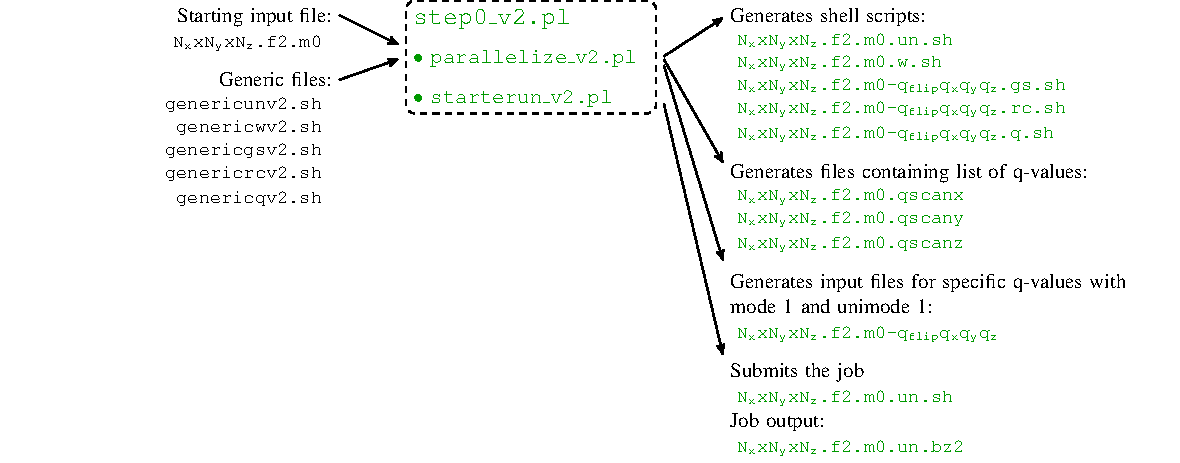
\includegraphics[scale =0.9]{perlflow/perlflow0.pdf}}
				  	\vspace*{0.25cm}
	\end{minipage}
	
	\begin{minipage}{\linewidth}
			\makebox[\linewidth]{
			 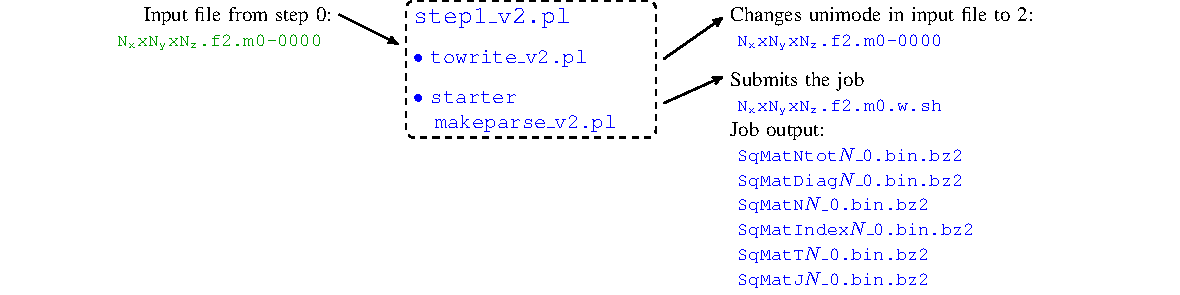
\includegraphics[scale = 0.9]{perlflow/perlflow1.pdf}}
			 	\vspace*{0.25cm}
	\end{minipage}
	
	\begin{minipage}{\linewidth}
			\makebox[\linewidth]{
			 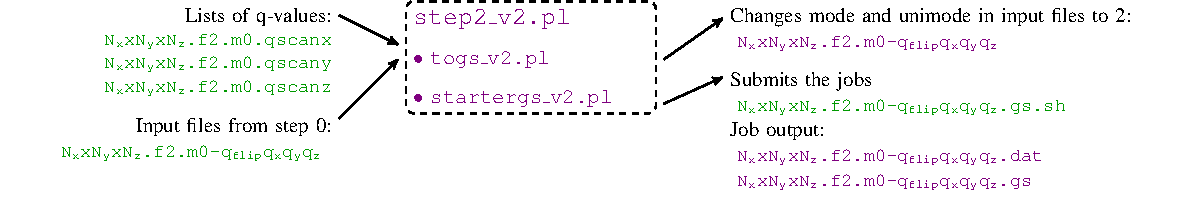
\includegraphics[scale = 0.9]{perlflow/perlflow2.pdf}}
			 	\vspace*{0.25cm}
	\end{minipage}
	
	\begin{minipage}{\linewidth}
			\makebox[\linewidth]{
			 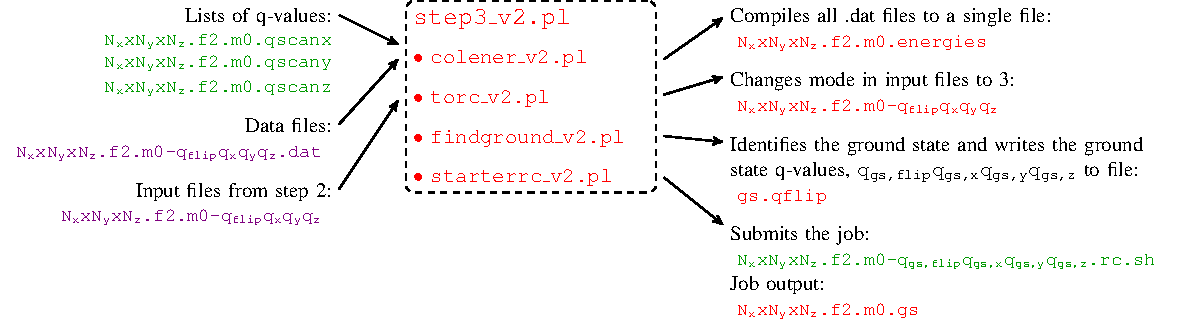
\includegraphics[scale = 0.9]{perlflow/perlflow3.pdf}}
			 	\vspace*{0.25cm}
	\end{minipage}
	
	\begin{minipage}{\linewidth}
			\makebox[\linewidth]{
			 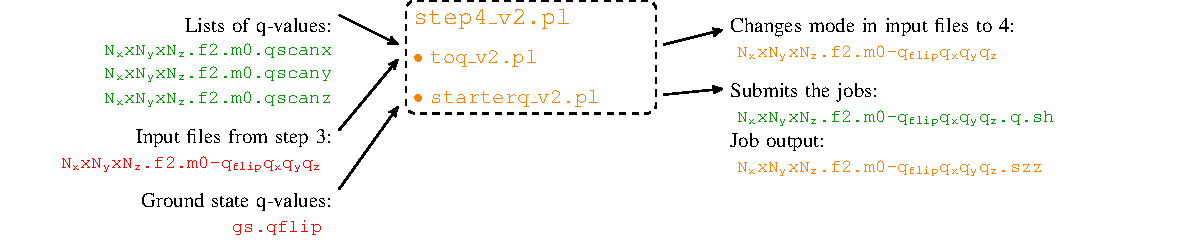
\includegraphics[scale = 0.9]{perlflow/perlflow4.pdf}}
			 	\vspace*{0.25cm}
	\end{minipage}
	\begin{minipage}{\linewidth}
			\makebox[\linewidth]{
			 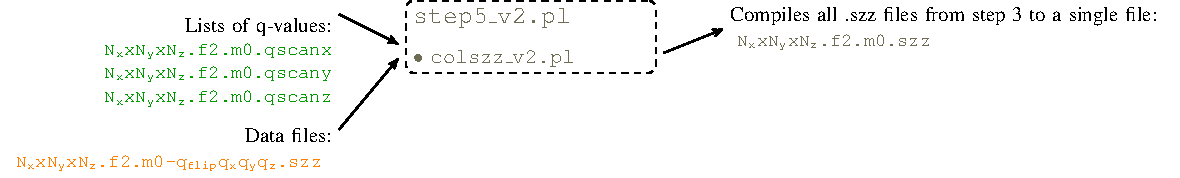
\includegraphics[scale = 0.9]{perlflow/perlflow5.pdf}}
			\captionof{figure}{Overview of the perl layer. The input of the different subroutines are listed in the left column, while the output are listed in the left. The example file names have been done for a system of arbitrary size in the $m = 0$ subspace. For any other $m$-subspace the zeroes of the file names would have to be changed to $2 \cdot \texttt{mval}$. Figures from \cite{CBL}. Please see section \ref{sec:generic} for details on the generic files, and how to handle error messages from the cluster.}
			\label{fig:perlflow}
				\vspace*{0.25cm}
	\end{minipage}
	
	
	\vspace*{0.5cm}	
	
	The steps can run together by using the Stepall. This step essentially only performs bookkeeping, and then runs the other steps at the correct time. Firstly it removes all files for the given system from previous runs. Then it runs each step, and checks that the required files are present before running the next step. Step\_all is run in the console by typing \texttt{./Stepall\_v2.pl} followed by a list of arguments. This is for example done for step 0 below.
	\begin{equation*}
		\texttt{./stepall\_v2.pl N$_\texttt{x}$ N$_\texttt{y}$ N$_\texttt{z}$ N geo spinflip msym mval}
	\end{equation*}
	Each step can also be run individually using the above formula, simply substituting the call to another step file. The same list of arguments is used for all of the different steps. These arguments are defined as follows:
	\begin{itemize}
		\item \texttt{N$_\texttt{x}$}, \texttt{N$_\texttt{y}$} and \texttt{N$_\texttt{z}$} describe the size of the finite lattice. For a chain of four spins this would simply be (\texttt{N$_\texttt{x}$}, \texttt{N$_\texttt{y}$}, \texttt{N$_\texttt{z}$}) = (4 1 1). In the case of the simple 4 $\times$ 4 lattice the answer is (\texttt{N$_\texttt{x}$}, \texttt{N$_\texttt{y}$}, \texttt{N$_\texttt{z}$}) = (4 4 1).
		\item \texttt{N} describes the total number of spins in the finite lattice, typically this would be \texttt{N}  = \texttt{N$_\texttt{x}$}  $\times$ \texttt{N$_\texttt{y} $  $\times$ \texttt{N$_\texttt{z} $}}.
		\item \texttt{geo} is a parameter used to indicate the system geometry, and is used to create the lists of $\textbf{q}$-values to scan over. If \texttt{geo}=0 the assumed geometry is a one-dimensional chain. The $q_x$ list will in this case contain the integer values from 0 to \texttt{N$_\texttt{x}$}/2, while the $q_y$ and $q_z$ lists will purely contain zeroes. If \texttt{geo} = 1 the assumed geometry is a square lattice, and the scanned q-values will correspond to the distinct $\textbf{q}$-values of the first Brillouin zone. A value of \texttt{geo} = 2 corresponds to a custom symmetry, where the lists of $\textbf{q}$-values to be scanned over will have to be created manually. 
		\item \texttt{spinflip} determines whether or not spinflip symmetry should be applied to the calculations. A value of \texttt{spinflip} = 2 means that spin flip symmetry should be applied, while \texttt{spinflip} = 1 means that it should not. 
		\item  \texttt{msym} is used to decide whether $m$-symmetry should be applied to the calculations. If \texttt{msym} = 1, the symmetry is applied, while it is not if \texttt{msym} = 0.
		\item If the calculations are done with $m$-symmetry, one should also define the $m$-subspace that they are done in. This  is defined through the parameter \texttt{mval}, which can take any value from 0 to \texttt{N$_\texttt{tot}$}/2. 
	\end{itemize}
	Of course, in order to solve a system using for instance m-symmetry, the RLexact files must be compiled with this flag turned on first. Otherwise \texttt{Stepall\_v2.pl} will give helpful error messages.\\
	 
	As an example, in order to run stepall for a $20 \times 1$ chain in the $m = 0$ subspace with spin flip symmetry, one would have to type the following command:
	\begin{equation*}
		\texttt{./stepall\_v2.pl 20 1 1 20 0 2 1 0}
	\end{equation*}
	A square $4 \times 4$ system without spin flip and without m-symmetry would be obtained by running:
	\begin{equation*}
		\texttt{./stepall\_v2.pl 4 4 1 16 1 1 0}
	\end{equation*}
	
By invoking this command the system looks for a given model file containing all the details: the spin couplings, the applied field, the exchange coupling etc. In order for the Perl layer to find this file it must be named specifically. For the $20 \times 1$ chain above, the program will look for a file called \texttt{20x1x1.f2.m0} - the \texttt{f} refers to the spin flip parameter, and \texttt{m} refers to the fact that m-symmetry is included and only $m=0$ should be investigated. For the $4 \times 4$ system, the program will look instead for a file called \texttt{4x4x1.f1.h}. Again \texttt{f} refers to the spin flip parameter, while \texttt{h} means that no m-symmetry is used, and that magnetic fields can be included.\\

The programme only works when 3 custom symmetries are given. The first symmetry must be an identity symmetry: if spin-flip symmetry is included this replaces the identity symmetry. Next comes the translation symmetries requested. An example for a model files of a $4 \times 1$ chain without spin flip symmetry in a magnetic field can be seen below. \\

If one wishes to sweep over a range of magnetic fields, this can be done using an additional over-overlayer called \texttt{steph\_v2.pl}. This step does not take any arguments, as opposed to the other files. The commands normally given to the other step files must be entered into the file in the top and it requires the following commands:
\begin{lstlisting}
$filename= '4x1x1.f1.h';
$command = '4 1 1 4 0 1 0';
@field=(0.2, 0.8);
\end{lstlisting}
If one inputs these lines, then \texttt{steph\_v2.pl} changes the field value in the file given by \texttt{\$filename} to the required field values given in \texttt{\$field}, and runs RLexact for each value. The energies and dynamical correlation functions are then saved in \texttt{\$filename\_master} files.

\subsection{\texttt{4x1x1.f1.h}}
\begin{lstlisting}
Ritz_conv 0.0000001 
Zero_vec_length 0.000001
Mode 0 //mdt
Unimode 0 //mdt
M start 0
M end 0
Number of spins 4 
Number of Couplings 4 
Number of Couplingstrengths 1
Number of Hardcoded symmetries 0 // 1 if spinflip-sym is used - otherwise 0. 
Number of custom symmetries 3  
Number of chosen GS q-values 0 //0 if we wish to look in all q-subspaces
Dimensions 1
Translation vector 1
Spin position 0
Spin position 1
Spin position 2
Spin position 3
Number of structurefactors 2
Q vector 0 1
Construct symmetries 0
Hardcoded symmetries 0
Custom symmetry 0 1 2 3
Custom symmetry 1 2 3 0
Custom symmetry 0 1 2 3
Number of chosen symmetries 0
Hx 1
Hy 0
Hz 0
H start 0.8
H step 1 //cannot be zero
H end 0.8
Coupling strength vector 1 1 0 // Given as (J_z, (J_x+J_y)/2, (J_x-J_y)/2 )
Coupling vector 0 1 0
Coupling vector 1 2 0
Coupling vector 2 3 0
Coupling vector 3 0 0
\end{lstlisting}

\subsection{A note on \texttt{generic} files}
\label{sec:generic}
As can be seen in figure \ref{fig:perlflow} many of the steps make use of so-called \texttt{generic} files. These files contain the commands needed to take a given job, send it along to the cluster nodes using the SLURM interface of the DCSC cluster, and then bring back the desired result files.  All files contains the following lines as the first lines (possibly with changed numbers):
\begin{lstlisting}
#!/bin/sh
#SBATCH -o /lustre/hpc/others/[user]/scratch/job1.%j.out
#SBATCH -e /lustre/hpc/others/[user]/scratch/job1.%j.err
#SBATCH --time=72:00:00
#SBATCH --partition=others
#SBATCH --ntasks=1
#SBATCH --mem=15G
#SBATCH --tmp=80G
\end{lstlisting}
The first two lines contains a reference to the directory that SLURM should direct output messages and error messages, \textbf{and it is important to change these directory to be subdirectories of your own user on the cluster} - this must be changed for all 5 \texttt{generic} files. Additionally, the \texttt{generic} files contains information on the maximum allowed time (in hh:mm:ss), which partition it is on, how many parallel task a given job has (which is always 1), and then the requested number of memory and temporary space. These can be changed if one needs to run exceptionally large systems.


\section{Plans for package upgrades}
Foreseen upgrades are given in the list below
\begin{itemize}
\item Include 4-spin ring exchange (done, describe it in the manual.)
\item Include dipolar interaction (previous version of the project had that)
\item Allow also systems without periodic boundary conditions
\end{itemize}

\section*{Acknowledgements}
First of all, I like to thank my collaborator through decades, Christian Rischel, without whom this project certainly would never have happened. In addition, I like to thank my US collaborators Collin Broholm, Daniel Reich, and Daniel Dender, who gave me the initial inspiration to the first version of the program.

Thanks to the students who have used RLexact as a part of their B.Sc., M.Sc. or Ph.D. work: 
Jacob Ibsen, Karen-Anne Herdal, Heidi Kolmorgen Nielsen, Torsten-Tranum-R\o mer, Kirsi I. Juntunen, 
Astrid Tranum-R\o mer, Turi K. Sch\"affer, Ellen Fogh, Camilla Buhl Larsen, and Erik Dreier Christensen, and Sofie Janas.

In addition, the students Frederik Treue and Bjarke M\o nsted were of invaluable help during the porting of the code to the DCSC cluster.

\begin{thebibliography}{99}
\bibitem{lefmann96} K. Lefmann and C. Rischel, Dynamical Correlation functions of the Nearest Neighbor and Haldane-Shastry Heisenberg Antiferromagnetic $s=1/2$ chains in zero and applied fields, Phys. Rev. B {\bf 54}, 6340-50 (1996) 
\bibitem{rischel98} C. Rischel and K. Lefmann, Magnetic order of $s=1/2$ spins on the FCC lattice at zero temperature calculated by exact diagonalization, J. Magn. Magn. Mater., {\bf 177-181}, 775-776 (1998) 
\bibitem{lefmann00} K. Lefmann, J. Ipsen, and F. B. Rasmussen, Thermodynamics of Rh nuclear spins calculated by exact diagonalization, Physica B {\bf 284}, 1702-1703 (2000) 
\bibitem{lefmann01} K. Lefmann and C. Rischel, Quantum effects in magnetic structures on the fcc lattice, Europ. Phys. J. B {\bf 21}, 313-329 (2001)
\bibitem{juntunen01} K. I. Juntunen, K. Lefmann, T. A. Knuuttila, and J. T. Tuoriniemi, High-temperature expansion and exact diagonalisation of the rhodium nuclear spin system compared to experimental results, J. Low Temp. Phys. {\bf 124}, 271-289 (2001)
\bibitem{ronnow01} H. M. R\o nnow, D. F. McMorrow, A. Harrison, I. D. Youngson, R. Coldea, T. G. Perring, G. Aeppli, O. Syljuasen, K. Lefmann, and C. Rischel, Spin dynamics of the 2D spin 1/2 anti-ferromagnet copper deuteroformate tetradeuterate (CFTD), Phys. Rev. Lett. {\bf 87}, 037202 (2001) 
\bibitem{ronnow02} H. M. R\o nnow, D. F. McMorrow, R. Coldea, A. Harrison, I. D. Youngson, T. G. Perring, G. Aeppli, O. Syljuasen, K. Lefmann, and C. Rischel, Comment on “Spin dynamics of the 2D quantum antiferromagnet copper deuteroformate tetradeuterate (CFTD)” - Reply, Phys. Rev. Lett. {\bf 89}, 079702 (2002)
\bibitem{zhang02} N.-G. Zhang, C. J. Henley, C. Rischel, and K. Lefmann, Effective Hamiltonian and low-lying eigenenergy clustering patterns of four-sublattice antiferromagnets, Phys. Rev. B {\bf 65}, 064427 (2002) 
\bibitem{stone03} M.B. Stone, D.H. Reich, C. Broholm, K. Lefmann, C. Rischel, C.P.  Landee, and M.M. Turnbull, Extended quantum critical phase in a magnetized spin-1/2 antiferromagnetic chain, Phys. Rev. Lett. {\bf 91}, 037205 (2003) 
\bibitem{fogh15} E. Fogh, T.K. Sch\"affer, A. Tranum-R\o mer, B. M\o nsted, and K. Lefmann,
Two- and four-spin excitations in the 1-dimensional nearest neighbour quantum Heisenberg antiferromagnet,
in preparation (2015)
%\bibitem{}
\bibitem{HKA} Heidi K.\ Nielsen and Karen-Anne Herdal, {\em Magnetic Bloch Oscillations}, M.Sc. thesis, 
   IMFUFA, University of Roskilde (2003)
\bibitem{TTR} Torsten Tranum-R\o mer, 
{\em Numerical studies on the Heisenberg antiferromagnet on a square lattice}, 
M.Sc. thesis, Niels Bohr Institute, University of Copenhagen (2010)
\bibitem{ATR} Astrid Tranum-R\o mer, 
Ph.D. project, Niels Bohr Institute, University of Copenhagen (2015)
\bibitem{CBL} Camilla Buhl Larsen, 
{\em Quantum Magnetism}, 
M.Sc. project, Niels Bohr Institute, University of Copenhagen (2015)
\bibitem{EDC} Erik Dreier Christensen, 
{\em Quantum Magnetism}, 
M.Sc. project, Niels Bohr Institute, University of Copenhagen (2015)
\bibitem{ring} Larsen, C. B., R\o mer, A. T., R\o mer, T. T., R\o nnow, H. M., and Lefmann, K. Concomitant Neel and RVB order in the low-energy spectrum of the Heisenberg quantum antiferromagnet on the square lattice. Submitted to PRB (2018).
\bibitem{SJ} Sofie Janas, M.Sc. project, Niels Bohr Institute, University of Copenhagen (2017)
\end{thebibliography}

\newpage
\appendix
\section{Structure of the RLexact C code}
RLexact is written in ANSI-C, but compiled with a C++ compiler. Therefore all files have extension ''.C``

The code is divided into a number of files, each containing a number of C functions representing a specific task of the program: main program, initialization, diagonalization, I/O, etc. The names of these files are shown in Table~\ref{tab:files}.

\begin{table}
\begin{tabular}{|l|l|} \hline
File name & Explanation \\ \hline
RLexact.h & Header file, definitions for all C files  \\
RLexact.C & Main program, controls program flow \\
RLio.C & Cares for all I/O function, including input file  \\
RLtables.C & Cares for initialization and storage of tabulated information  \\
RLsymm.C & Calculates the symmetry operations \\
RLhamil.C & Calculates the effect of the Hamiltonian on a state \\
RLsparse.C & Controls the storage of the sparse Hamiltonian matrix \\
RLmatrix.C & Performs Matrix diagonalization \\
RLlancz.C & Performs Lanzcos diagonalization \\
RLcross.C & Calculated cross sections \\
RLutil.C & Different general usesul functions \\
nr.C & Routines from Numerical Recipes \\
regc.cpp & ??? \\
Diagonal.C & Diagonalizes complex hermitean matrices, adapted from Numerical Recipes \\
\hline
\end{tabular}
\caption{An overview of the files that constitute RLexact.} \label{tab:files}
\end{table}

Below, we discuss the structure of the functions in each of these files

\subsection{Structure of definitions in RLlancz.h}
This include file contains declaration of constants, complex math, excecution flags, verbose flags, and debug flags in RLexact. It also defines abbreviations of some inportant code parts.

Some of the constants are upper limits for array sizes, used in declarations. If needed, these values can be modified. The constants are \verb+MAXARRAYSIZE+, \verb+NSPINS+, \verb+NCOUP+, \verb+NRING+, \verb+NCOUPSTR+, \verb+NRINGSTR+, \verb+NSYM+, \verb+NSYMADD+, \verb+NUNIQUE+.

Some constants are defined automatically on the basis of the other constants and should not be modified:
\verb+MAX_STATE+.

Some constant are extentions to the C math:
\verb+PI+, \verb+SQR(a)+.

Other constants control the operation of the excecution:
\verb+BUFFERSIZE+, \verb+RITZ_CONV+, \verb+ZERO_VEC_LENGTH+  (ARE THEY USED???), \verb+SHORT_VEC_LENGTH+, \verb+MAX_LANCZOS+, \verb+SMALL_NUMBER+, \verb+LARGE_NUMBER+, \verb+RANDOM+, \verb+SPIN_0_UP+.

Some constants are concerned with filenames:
\verb+FILEEND+, \verb+LOGFILEEND+, \verb+SZZEND+, \verb+SPMEND+, \verb+SMPEND+, \verb+MATRIXFILENAME+, \verb+COEND+, \verb+GSCOEND+, \verb+UNIEND+, \verb+UNIOBSEND+.

Finally, some constants are just marking options:
\verb+MASK_L1+, ... \verb+MASK_L4+, \verb+MASK_P1+, \verb+MASK_P2+, \verb+SPIN_FLIP+, \verb+FCC32Tx+, \verb+FCC32Ty+, \verb+FCC32Tz+, \verb+FCC32MIRROR+, \verb+FCC32R2+, \verb+FCC32R4+, \verb+FCC32R3+, \verb+IDENTITY+, \verb+LINEAR_T+, \verb+START+, \verb+STOP+, \verb+X+, \verb+Y+, \verb+Z+, \verb+REAL+, \verb+IMAG+, \verb+NORMAL+, \verb+RECONSTRUCT+, \verb+CROSS+, \verb+SZZ+, \verb+SPM+, \verb+SMP+, \verb+MODEN+, \verb+MODEGS+, \verb+MODEQ+, \verb+UNIMODEEN+, \verb+UNIMODEW+, \verb+UNIMODER+.

The complex math parts can be seen as an extension of the C language. If \verb+USE_COMPLEX+ is not set, the following are replaced by real-number math:
\verb+komplex+, \verb+kvector+, \verb+freekvector+, \verb+kmatrix+, \verb+freekmatrix+, \verb+I+, \verb+zero+, \verb+one+, \verb+Arg(a)+, \verb+arg(a)+, \verb+abs(a)+, \verb+sqrabs(a)+, \verb+eksp(a)+, \verb+conj(a)+, \verb+skrt(a)+.

The excecution flags are
\begin{itemize}
\item \verb+MSYM+ allows for the use of $m$-value symmetry in the diagonalization
\item \verb+DIPOLE+ allows for dipole interaction
\item \verb+LANCZOS+ makes RLexact diagonalize by the Lanczos algorithm
\item \verb+MATRIX+ makes RLexact diagonaliza by direct matrix methods
\item \verb+STRUCTURE+ (FIND OUT WHAT THIS DOES!)
\item \verb+USE_COMPLEX+ allows for the use of complex numbers in the diagonalization (should be set unless you are really sure what you are doing!)
\end{itemize}

The code parts are: 
\verb+right(i)+, \verb+inverse(i)+, \verb+symnun(i,j)+, \verb+TLOOP_BEGIN+, \verb+TLOOP_END+, \verb+TRANSLOOP_BEGIN+, \verb+TRANSLOOP_END+, \verb+QLOOP_BEGIN+, \verb+QLOOP_END+

All verbose flags start with \verb+VERBOSE+ and logs timing- and other mesages to the log file during excecution. 
Verbose flags can be set even if large systems are diagonalized. (MAKE THIS HAPPEN!)

All debug flags start with \verb+TEST_+ and prints debug messages to the log file. Diagonalization of system with 
$N>10$ should not be performed when any debug flag is set.


\subsection{Structure of main program and functions found in RLexact.C}
This file contains the main program \verb+main()+, which controls the main program flow and is explained below.
The file also contains the functions \verb+Solve_Lanczos()+ and \verb+Solve_Matrix()+, which takes care of the cases of Lanczos 
and matrix diagonalization, respectively. Also these two functions are sketched below.

\paragraph{Structure of main()} The basic structure of the main program is
\begin{itemize}
\item Print start message and read input file, \verb+RLio.C/intro()+
\item Fill in tables to use in calculations, \verb+RLtables.C/Build_Tables()+
\item Initialize symmetry calculations, \verb+RLsymm.C/InitSym()+
\item Identify and count unique states, \verb+RLtables.C/FillUnique()+
\item Allocate memory for the calculation, \verb+RLutil.C/allocate()+
\item Loop over all $m$-values, \verb+{+
\item \hspace{5mm} Identify and catalogue unique states for this $m$-value, \verb+RLtables.C/FillUnique()+
\item \hspace{5mm} Calculate observables for the uniques, \verb+RLtables.C/FillUniqueObservables()+
\item \hspace{5mm} Diagonalize the problem, \verb+RLexact.C/Solve_Lanczos()+ OR \verb+RLexact.C/Solve_Matrix()+
\item \verb+}+
\item \verb+RLio.C/outro()+
\item Free allocated memory, \verb+RLutil.C/deallocate()+
\end{itemize}

\paragraph{Structure of Solve\_Lanczos():} The basic structure of this function is
\begin{itemize}
\item Write sparse Hamiltonian matrix to file, \verb+RLsparce.C/MakeSparse()+
\item Loop over (all OR selected) $q$-values, \verb+{+
\item \hspace{5mm} Initialize for the particular $q$-value, \verb+RLtables.C/BuildCycle()+
\item \hspace{5mm} Perform Lanzcos diagonalization, \verb+RLlancz.C/LowestLanczos()+
\item \hspace{5mm} Write results fo file, \verb+RLio.C/WritehmQ()+ AND \verb+RLio.C/WriteResults()+
\item \hspace{5mm} IF minimum energy here is lower than previous, THEN store this value and the $q$-value
\item \verb+}+
\item Possibly write ground state to disk, \verb+RLio.C/WriteState()+
\item Initialize for the $q$-value of the ground state, \verb+RLtables.C/BuildCycle()+
\item Calculate $S^{zz}(q,\omega)$ from the ground state, \verb+RLlancz.C/CrossLanczos()+
\item Loop over ALL $q$-values, \verb+{+
\item \hspace{5mm} Initialize for the current $q$-value, \verb+RLtables.C/BuildCycle()+
\item \hspace{5mm} Calculate $S^{zz}(q,\omega)$, \verb+RLlancz.C/CrossLanczos()+
\item \verb+}+
\end{itemize}
I CANNOT UNDERSTAND WHAT HAPPENS BEFORE THE LAST LOOP, SOME FUNCTIONALITY SEEMS REPEATED!

!CLARIFY DIFFERENCE BETWEEN STATE $q$ AND THAT OF $S(q,\omega)$! PERHAPS DIFFERENT NOTATION!?

\paragraph{Structure of Solve\_Matrix():} The basic structure of this function will not be described now...


\subsection{Structure of functions found in RLio.C}
The file \verb+RLio.C+ contains all functions related to input/output in RLexact. No write statements (e.g. \verb+printf()+)
should be present in other files. One exception is the temporary storage of tables on file, controlled in \verb+RLtables.C+.

\verb+RLio.C+ contains the functions that presents the opening and closing messages, \verb+intro()+ and \verb+outro()+, respectively.
It contains the important function that reads and interprets the input file, \verb+ReadCoupPattern()+.
The latter function has the subfunctions \verb+TransformCoup()+ and \verb+FillRotationMatrix()+ to transform the data from the input file in the case of an applied field where the coordinate system is rotated to have the z-axis along the field.

\verb+RLio.C+ contains functions that writes calculation results to file: \verb+writemaggs()+, \verb+WriteState()+, \verb+WritehmQ+, \verb+WriteResults()+, \verb+WriteCross()+, \verb+WriteGSEnergy()+, \verb+WriteEnergy()+, \verb+WriteGSdata()+. It also contains
the function to read ground state data from file, \verb+ReadGSdata()+.

\verb+RLio.C+ also contains functions that perform debug- and other user messages: \verb+Warning()+, and \verb+Message_*()+, and it has the function that performs the timing of calculations, \verb+time_stamp()+. It also has the function that halts the system: \verb+fatalerror()+.

TODO: separate debug- and other messages.

\paragraph{Structure of intro():} The basic structure of the introduction function is 
\begin{itemize}
\item Print RLexact welcome message
\item Print the current set-up of RLexact
\item Input the name of the infile from the command line
\item Generate the names of the output files
\item Open the output files
\item Read and interpret the input file, \verb+RLio.C/ReadCoupPattern()+
\end{itemize}

\paragraph{Structure of outro():} The basic structure of the short exit function is 
\begin{itemize}
\item Close the output files
\item Print RLexact exit message
\end{itemize}

\paragraph{Structure of ReadCoupPattern():} The basic structure of the important input file reader is 
\begin{itemize}
\item Open and read the input file
\item Read the running modes, \verb+Mode+ and \verb+Unimode+
\item Possibly read the control parameters for the Lanczos algorithm, \verb+Ritz_conv+ and \verb+Zero_vec_length+
\item Read the basic parameters for the interactions, \verb+Nspins+, \verb+Ncoup+, \verb+Ncoupstr+, \verb+Nring+, \verb+Nringstr+
\item Read the basic parameters for the symmetries, \verb+Nsym+, \verb+Nsymadd+, \verb+symconstruct+
\item Possibly read the number of $q$-values to look for the ground state, \verb+Nq_choice+, and read these $q$-values 
\item Possibly read the positions of the spins, the number of spatial $q$-values to calculate $S({\bf q},\omega)$, \verb+Nstruct+ 
- and these $q$-values.
\item Either read the range of $m$-values or the range and direction of $h$-values
\item Read the pair couplings strengths - and the spin pairs that interact
\item Read the ring coupling strengths - and the spin rings that interact
\item Possibly construct the coupling scheme from the symmetries present, \verb+MakeSymCoup+ (DOES NOT WORK) 
\end{itemize}

TODO: Implement in the Perl layer that you may choose the $q$-values for the GS search, like it is done when run from command line!

\subsection{Structure of functions found in RLtables.C}
The file \verb+RLtables.C+ contains functions that are concerned with the use of tables to ease the diagonalization calculations. 
Included in this is the storage of tables to file.

The file countains the main function \verb+Build_Tables()+ that controls the filling of tables at program start, as well as the two functions \verb+FillUnique()+ and \verb+FillUniqueObservables()+ that tabulates the unique states and their physical properties.

The communication with files is taken care of by \verb+ReadUnique()+, \verb+ReadUniqueObservables()+, \verb+WriteUnique()+, and \verb+ReadUniqueObservables()+.

In addition, a number of functions perform minor tasks: \verb+Count()+, \verb+BuildCycle()+, \verb+FindUnique()+, \verb+IsUnique()+, and \verb+LookUpU()+.

\paragraph{Structure of BuildTables():} The basic structure of this important function in \verb+RLtables.C+ is
\begin{itemize}
\item Tabulate trigonometric functions, $\cos(2\pi j / N_{\rm spins})$ and $\sin(2\pi j / N_{\rm spins})$, 
for $j=0$ to $N_{\rm spins}-1$.
\item Tabulate square root function, $\sqrt{j}$, for $j=0$ to $2(N_{\rm spins}+1)N_{\rm spins}$. TODO: CHECK IF THIS IS A TOO HIGH LIMIT
\item Possibly: calculate the total phase factor from the chosen q-values for each lattice site. TODO: CHECK IF THIS WORKS!  
\end{itemize}

\paragraph{Structure of FillUnique():} This function finds and counts all uniques and, if the flag \verb+CountOnly+ is not set, fills the tables of unique states. The basic structure of this important function in \verb+RLtables.C+ is
\begin{itemize}
\item IF $m$ is a good quantum number
\item \hspace{5mm} Loop over all states with magnetisation $m$ (special algorithm working only for $s=1/2$)
\item ELSE
\item \hspace{5mm} Loop over all states \{
\item \hspace{10mm} IF the state is unique, \verb+IsUnique()+ THEN count and possibly register the state
\item \hspace{5mm} \}
\end{itemize}

\paragraph{Structure of FillUniqueObservables():} The basic structure of this important function in \verb+RLtables.C+ is
\begin{itemize}
\item Loop over all unique states \{
\item \hspace{5mm} Register the magnetization, \verb+Count()+
\item \hspace{5mm} Calculate $S^{zz}(q)$ and register it
\item \}
\end{itemize}

\paragraph{Structure of BuildCycle():} This function finds the repetition period of a unique under the different symmetry operations for a particular value of \verb+q[]+. The basic structure of this function in \verb+RLtables.C+ is
\begin{itemize}
\item Loop over all unique states, from the table \verb+unique[]+ \{
\item \hspace{5mm} Run through all combinations of symmetry operations, from zero to $N-1$ times each. \{
\item \hspace{10mm} count the number of times the particular unique is encountered 
\item \hspace{10mm} sum the complex phase of all occurences of the unique
\item \hspace{5mm} \}
\item \hspace{5mm} For consistency, check that the number of occurences is an integer fraction of the number of symmetry possibilities and that the imaginary part of the complex phase is zero.
\item \hspace{5mm} IF the real part of the complex phase is non-zero (the unique is realized at that particular value of \verb+q[]+) THEN count and register this unique.
\item \}
\end{itemize}

\subsection{Structure of functions found in RLsymm.C}
The file \verb+RLsymm.C+ contains functions that are concerned with the initialization and use of symmetry functions, including tables  concerned with symmetry. It also contains the  functions \verb+SymOpSite+ and \verb+MakeSymCoup+, which are used for a feature in development, as well as the function \verb+TestSym+, used only for debugging.

\paragraph{Structure of SymOp():} This function performs a given symmetry operation on a unique state and returns the result.
\begin{itemize}
\item Recognize the symmetry operation
\item Perform the symmetry operation on the input state
\item Return the result
\end{itemize}

\paragraph{Structure of InitSym():} This function initializes the tables of symmetry operations
\begin{itemize}
\item Loop through all chose symmetries; both hard coded and added \{
\item \hspace{5mm} Find and register the maximum period of that symmetry; (CHECK ONCE MORE WHICH VARIABLES ARE UPDATED)
\item \}
\end{itemize}

\subsection{Structure of functions found in RLhamil.C}
We will not write this now, as it is subject to change

\subsection{Structure of functions found in RLsparse.C}
This file contains functionality related to the implementation of sparse matrices in RLexact.
It contains only two functions, \verb+MakeSparse()+ to write the sparse Hamiltonian matrix to file, and \verb+ApplySparse()+ to read it from file and apply it to a given state vector.

\paragraph{Structure of MakeSparse():}
This function identifies non-zero matrix elements of the sparse Hamiltonian and writes this to a file.
\begin{itemize}
\item Generate file names and open the 5 files: \verb+indexfile+, \verb+Jfile+, \verb+Tfile+, \verb+nelemfile+, \verb+diagfile+.
\item Loop over all uniques, $i$ \{
\item \hspace{5mm} Calculate the diagonal element of $H$
\item \hspace{5mm} Loop over all 2-spin off-diagonal coupling terms in H, $j$ \{
\item \hspace{10mm} Generate a new state from $H_{2,j} |i\rangle $
\item \hspace{10mm} Find the corresponding new\_unique
\item \hspace{10mm} If new\_unique is allowed for this $k[]$ \{
\item \hspace{15mm} if upper triangle in matrix, write coupling and strength to files
\item \hspace{10mm} \}
\item \hspace{5mm} \}
\item \hspace{5mm} Write diagonal element to files
\item \}
\item Close the 5 files
\end{itemize}

\paragraph{Structure of ApplySparse():}
This function reads the sparse Hamiltonian from file and applies that to a state, \verb+vectin+, returning a new state, \verb+vectout+.

\begin{itemize}
\item Generate file names and open the 5 files: \verb+indexfile+, \verb+Jfile+, \verb+Tfile+, \verb+nelemfile+, \verb+diagfile+.
\item Initialize \verb+vectout+ to zero.
\item Loop over all uniques, $i$ \{
\item \hspace{5mm} Read diagonal element of $H$
\item \hspace{5mm} Update \verb+vectout+ with the diagonal term
\item \hspace{5mm} Loop over all sparse off-diagonal coupling terms of H, \verb+j+ \{
\item \hspace{10mm} Read coupling term \verb+j+
\item \hspace{10mm} Calculate the phase $T \cdot k$, and the corresponding actual coupling strength
\item \hspace{10mm} Update \verb+vectout+ with one off-diagonal term - and with its Hermitean conjugate
\item \hspace{5mm} \}
\item \}
\item Close the 5 files
\end{itemize}

\subsection{Structure of functions found in RLmatrix.C} 
Functions in this file performs diagonalization using exact matrix method. It will be described later.

\subsection{Structure of functions found in RLlancz.C} 
The functions in this file takes care of running the Lanczos diagonalization algorithm.

TODO: The file contains two functions, \verb+findmag+ and \verb+findmaggs+, which are doubtful and should be checked.

\paragraph{Structure of LowestLanczos():} This function performs the main control of the Lanczos algorithm.
\begin{itemize}
\item Determine the Lanzcos seed by call of \verb+MakeSeed()+ or \verb+MakeSeedCross+, depending on the running mode.
\item Write seed vector to file
\item Set the first Lanczos vector equal the seed and reset the two other Lanczos vectors.
\item Perform the Lanczos diagonalization by calling \verb+LanczosLoop()+ with first argument zero.
\item Record energy and magnetization of the found states
\item IF requested THEN record the structure factor $S(q)$ on the ground state. CHECK IF THIS WORKS!
\item Search for the Lanczos state with lowest energy
\item IF ground state requested THEN \{
\item \hspace{5mm} Reconstruct the Lanczos sequence
\item \hspace{5mm} Restore the Lanczos seed
\item \hspace{5mm} Redo most of the Lanczos diagonalization by calling \verb+LanczosLoop()+ with first argument nonzero.
\item \hspace{5mm} Calculate the magnetization of the ground state
\item \}
\end{itemize}

\paragraph{Structure of LanczosLoop():} This function performs the actual Lanczos algorithm. Most of the excecution time of RLexact is spent within the main loop of this function.
\begin{itemize}
\item WHILE stopping condition is not met \{
\item \hspace{5mm} If reconstruction mode, update the ground state with contribution from the current Lanczos vector
\item \hspace{5mm} Take one Lanczos step by call of \verb+NextLanczos()+
\item \hspace{5mm} Update Lanczos vectors 
\item \hspace{5mm} If not reconstruction mode, update the Lanczos matrix
\item \hspace{5mm} Evaluate stopping condition (CHECK IF THIS WORKS OPTIMALLY)
\item \}
\end{itemize}


\paragraph{Structure of NextLanczos():} This function performs one step of the Lanczos algorithm, by executing the following steps:
\begin{itemize}
\item Calculate $H|v_r\rangle$, by calling \verb+ApplySparse()+.
\item Calculate $|u_r\rangle = H|v_r\rangle - |v_{r-1}\rangle\langle v_{r-1} | H | v_r \rangle$
\item Calculate $\langle v_r | H | v_r \rangle$
\item Set the next Lanczos vector $|v_{r+1} \rangle$ equal $|u_r \rangle - |v_r\rangle \langle v_r | H | v_r$
\end{itemize}
CHECK HOW THIS WORKS! RISCHEL!

\paragraph{Structure of MakeSeed():} This function generates a seed vector for the Lanzcos algorithm to find the ground
state. The default mode gives a random seed.

\paragraph{Structure of MakeSeedCross():} Depending on the input, this function copies one of the states 
$S^{zz}_k |0 \rangle$, $S^{+-}_k |0 \rangle$, $S^{-+}_k |0 \rangle$ to the Lanczos start vector.

\subsection{Structure of functions found in RLcross.C}
\subsection{Structure of functions found in Diagonal.C}
\subsection{Structure of functions found in regc.cpp}
\subsection{Structure of functions found in nr.C}
The file \verb+nr.C+ contains a number of low-level functions, mostly concerned with allocating and de-allocating memory.
These functions are not discussed here.

\subsection{Structure of functions found in RLutil.C}
The file \verb+RLutil.C+ contains general-purpose and low-level functions, not belonging naturally in the other files:
\verb+reverse()+ reverses a string, \verb+itoa()+ converts an integer to a string, \verb+FillRotationMatrix()+ initializes a 3D rotation matrix, and \verb+RotateVector()+ utilizes the rotations matrix. The function \verb+Normalize()+ normalizes a komplex vektor. Finally \verb+Bubblesort()+ make a quick-and-dirty sort of a list.


\newpage
\section{The internal data structure}
\subsection{Variables controlled by the input file}
The data from the input file is stored in a number of variables in the RLexact, as shown in 
Table~\ref{tab:variables}.

\begin{table}
\begin{tabular}{|l|l|l|} \hline
Description & Variable & Maximal value \\
\hline
Number of spins & Nspins & NSPINS \\
Number of pair couplings & Ncoup & NCOUP \\
Number of different pair coupling strengths & Ncoupstr & NCOUPSTR \\
Number of hardcoded symmetry elements & Nsym & NSYM \\
Number of tablulated symmetry elements & Nsymadd & NSYMADD \\
Number of unique states & & NUNIQUE \\
Table of symmetries in use & symlist[] & \\
?? & **symadd & \\
Number of symmetry values used to finding the ground state & Nq\_choice & \\
Actual choices of symmetry values & q\_gs[NSYM] & \\
Coupling value $J^{zz}$ & Jzz[NCOUP] & \\
Coupling value $J^{xy}$ & Jxy[NCOUP] & \\
Coupling value $J^{\rm anis}$ & Janis[NCOUP] & \\
Coupling pair & hamil\_coup[NCOUP][2] & \\
Ring coupling value $J^{r}$ & Jr[NRING] & \\
Coupling ring & ring\_coup[NCOUP][4] & \\
\hline
\end{tabular}
\caption{An overview of the central variables and constants in RLexact.} \label{tab:variables}
\end{table}

\subsection{The RLexact.h file} \label{sect:RLexact.h}
The file RLexact.h defines dimensions of statically declared arrays in RLexact, as shown
in Table~\ref{tab:variables}. 

In addition, debug requests are defined here - too many possibilities to list in this manual.

\end{document}


